\documentclass[
11pt, % The default document font size, options: 10pt, 11pt, 12pt
%oneside, % Two side (alternating margins) for binding by default, uncomment to switch to one side
english, % ngerman for German
singlespacing, % Single line spacing, alternatives: onehalfspacing or doublespacing
%draft, % Uncomment to enable draft mode (no pictures, no links, overfull hboxes indicated)
%nolistspacing, % If the document is onehalfspacing or doublespacing, uncomment this to set spacing in lists to single
%liststotoc, % Uncomment to add the list of figures/tables/etc to the table of contents
%toctotoc, % Uncomment to add the main table of contents to the table of contents
%parskip, % Uncomment to add space between paragraphs
%nohyperref, % Uncomment to not load the hyperref package
headsepline, % Uncomment to get a line under the header
%chapterinoneline, % Uncomment to place the chapter title next to the number on one line
%consistentlayout, % Uncomment to change the layout of the declaration, abstract and acknowledgements pages to match the default layout
]{MastersDoctoralThesis} % The class file specifying the document structure


% Set the paths where to look for images
\usepackage{subcaption}
\graphicspath{{res/}{img/}}

\usepackage{amsmath}
\usepackage{styles/mdftheorems}

\begin{document}

\title{Application of machine learning, witch special focus on neural networks, for GPS satellite clock bias prediction.}


\author[PG]{Piotr Gny\'{s}}
\date{\today}


%----------------------------------------------------------------------------------------
%	OUTPUT TITLE PAGE AND PREVIOUS
%----------------------------------------------------------------------------------------

\maketitle


%----------------------------------------------------------------------------------------
%	TABLE OF CONTENTS & LIST OF FIGURES/TABLES
%----------------------------------------------------------------------------------------

\begingroup % Local scope for the following commands

% Define the style for the TOC, LOF, and LOT
%\setstretch{1} % Uncomment to modify line spacing in the ToC
%\hypersetup{linkcolor=blue} % Uncomment to set the colour of links in the ToC
\setlength{\textheight}{23cm} % Manually adjust the height of the ToC pages

% Turn on compatibility mode for the etoc package
\etocstandarddisplaystyle % "toc display" as if etoc was not loaded
\etocstandardlines % "toc lines as if etoc was not loaded

\tableofcontents % Output the table of contents

\listoffigures % Output the list of figures

% Comment both of the following lines to have the LOF and the LOT on different pages
\let\cleardoublepage\bigskip
\let\clearpage\bigskip

\listoftables % Output the list of tables

\endgroup


%----------------------------------------------------------------------------------------
%	MAIN BODY
%----------------------------------------------------------------------------------------

\chapter{Introduction}
FIXME : Textwidth in cm: \printinunitsof{cm}\prntlen{\textwidth}

%==================================================================================================
\section{Motivation}
I have encountered a problem that was insipration for this work during my research in field
of mobile robotics. While my initial focus was directed more towards emergent behaviour in 
robotics and a self organizing systems I have encountered a issue with localization in marine 
robotics. With high cost of internet connection for robots operating far away from land it 
is important to be able to calculate precise position without updating data from internet.
One of issuse when working with satellite navigation system is requirement for clock bias
correction, to keep error drift to minimum readouts for both local and satellite clock must
be corrected by predicted bias. In this work I focused on prediction of errors in satellite
clocks as unlike in case of local clock those can be later reused by other people.


%==================================================================================================
\section{Beacon based navigation in robotics}

%--------------------------------------------------------------------------------------------------
\subsection{Baisc concepts in robot localisation}

%--------------------------------------------------------------------------------------------------
\subsection{Radio beacon localisation}
All Global Satellite Navigation systems (GNSS) are variant of beacon-based localization
systems\cite{Blewitt1997}. Such systems require information about the beacon position
and distance between the localized object and beacons.
With that information, it is possible to calculate the position of an object in the same reference
frame as that of beacons.
Both of those tasks are much more difficult in GNSS due to the nature of the beacons.
Unlike in the case of stationary beacons, GNSS satellites move at high speed so
their position must be calculated based on satellite ephemerides.
Another problem is how to measure distance with use of reasonably priced reciever while 
maintaining high level of precision.
There are three possible approaches to a beacon based localisation:
\begin{itemize}
	\item Time of Arrival (ToA),
	\item Angle of Arrival (AoA),
	\item Received Signal Strength (RSS).
\end{itemize}
AoA detects at which angle a beacon signal arrives and reqires a specialised receiver capable 
of such measurements. This type of localization requires a complex reciever and do not provide 
a satisfactionary precision when dealing with such remote objects as a satellites.
While RSS can work with a very simple reciever its precision is low for signals that, like
the GPS signal, are designed with low power loss over large distances.
This leaves ToA as only valid solution, when measuring distance by ToA 
three properties of a signal should be known:
\begin{itemize}
	\item $t_o$ - time of origination,
	\item $t_a$ - time of arrival,
	\item $v$ - velocity.
\end{itemize}
In case of GNSS signal is an electromagnetic wave therefore its speed is equal
to a speed of light $c$. Time of arrival is recorded when
data frame wavefront reaches the receiver, this means that receiver time is used.
Signal generation time is recorded on satellite according to its local clock and
included in the data frame. Thanks to that distance can be calculated by simple
equation:
\begin{equation}
	d=c(t_a-t_o).
\end{equation}
However $t_a$ and $t_o$ are using different reference frame so for comparison
to be possible they must be transformed into a common reference frame.
This is referred to as a synchronization of the clocks and is very important as
a desynchronization on the level of a single nanosecond results in about 30 cm of
positioning error\cite{Enge2011}.

%--------------------------------------------------------------------------------------------------
\subsection{Global navigation satellite systems}






\chapter{Time metrology}
Aim of this chapter is to present an issue that will be dealt with in this work.
First a concept of theoretical clock will be presented alongside mathematical tools required
for it description and behavior modelling.
This is followed by a more detailed description of stability analysis which is most prominent
field of science dealing with clock behavior.
After describing theoretical clock models an attention will be given to physical implementation
of clock system with special focus on types of clocks used aboard GPS satellites.
Finally current state of the art in GPS clock bias prediction will be presented.
Intention of writing this chapter was that despite clock modelling and frequency analysis being
well known field readers with computer science might not be familiar with it.
For those well versed in frequency analysis most of this chapter can be safely skipped with 
exception of last section that focuses on state of the art in GPS clock prediction as it 
deals with issues that are more specific do described in this work.
It is important to understand that this chapter do not provide comprehensive knowledge about
described field as due to methodology used in presented work that knowledge it is not required.
For more information about clock modelling and stability analysis Handbook of Frequency Stability
Analysis is suggested as reading.


%====================================================================================================
\section{Physical clock implementation}
\label{sec:physical_clock}

%----------------------------------------------------------------------------------------------------
\subsection{Introduction to physical clock implementation}

%----------------------------------------------------------------------------------------------------
\subsection{Principles of atomic clock design}


%====================================================================================================
\section{Mathematical clock model}
In context of pure mathematical modelling a clock is understood as a function that describes
offset between two given values for a specific point in time. One of those values is referred 
to as the reference clock and it is considered to always return correct time $T_{r}(t)=t$.
It is important to understand that in physical systems value of $t$ is not only inaccessible, as
every measurement instrument have some degree of uncertainty, but do not exists at all.
This is due to time dilatation effect, derived from special theory of relativity, that causes
time to flow differently in systems that move with velocities close to speed of the light.
This issue is dealt with by selecting most precise physical clock available as the reference
clock and modelling difference between it and other clocks, including time dilatation effects,
as their bias.
Main goal of modeling clocks is to retrieve a value of $t$, which is equal to $T_{r}(t)$, based
on value read from given clock $T_{c}(t)$. 
As relation between those clock is fully described by analyzed clock bias 
$b_{c}(t)=T_{r}(t)-T_{c}(t)$ clock model is equivalent to just a bias model.

%----------------------------------------------------------------------------------------------------
\subsection{Discrete and continuous clock models}
There are two possible approaches to mathematical clock modelling, one of them is continuous
clock model that relies on differential equation for description of its behavior.
In this approach clock bias is modeled as :
\begin{equation}
	\label{equ:continous_clock}
	b_{c}(t) = T_{r}(t_{0}) +  \int_{t_{0}}^{t} \varepsilon_{c}(\tau) d\tau ,
\end{equation}
where:
\begin{itemize}
	\item $t$ is the independent time argument,
	\item $b_{c}(t)$ is the clock bias at time $t$,
	\item $t_{0}$ is time at which clock was synchronized with reference ($b_{c}(t_{0})=0$),
	\item $T_{r}(t_{0})$ is value of reference clock at $t_{0}$,
	\item $\varepsilon_{c}(\tau)$ is the normalized frequency offset of a clock.
\end{itemize}
The branch of science that deals with continuous clock modelling is called stability analysis.
In this work no more attention will be given to that approach as due to nature of data as well as
choice of prediction algorithms favour a discrete clock model.
In discrete clock model bias is described as :
\begin{equation}
	\label{equ:discrete_clock}
	b_{c}(i) = T_{r}(i) - T_{c}(i),
\end{equation}
where $i \in \mathbb{N}$ is the number of measurement.
One of main differences between continuous and discrete models is that in latter case bias is 
considered only as a difference between two individual measurements where in case of 
continuous model all differences starting from synchronization are taken into account.
Another important change is that in discrete model clock is a function $\mathbb{N} \to \mathbb{R}$
instead of $\mathbb{R} \to \mathbb{R}$ like it was in case of continuous model. 
This requires redefinition of reference clock from $T_r{t}=t$ into:
\begin{equation}
	\label{equ:discrete_reference}
	T_{r}(i) = \Delta T_r i,
\end{equation}
where $\Delta T_r$ is the measurement period of reference clock.
In such model $T_{r}$ as well as $T_{c}$ are time series which means that $b_{c}$ is also one.
This means that methodologies related to time series analysis like \textbf{TODO : LIST METHODS}
can be used.
Usually clocks are modelled as a linear combination of several deterministic and stochastic 
components as shown on Figure \ref{fig:clocks_example}. 
\begin{figure}[htb] 
\label{fig:clocks_example}
\centering
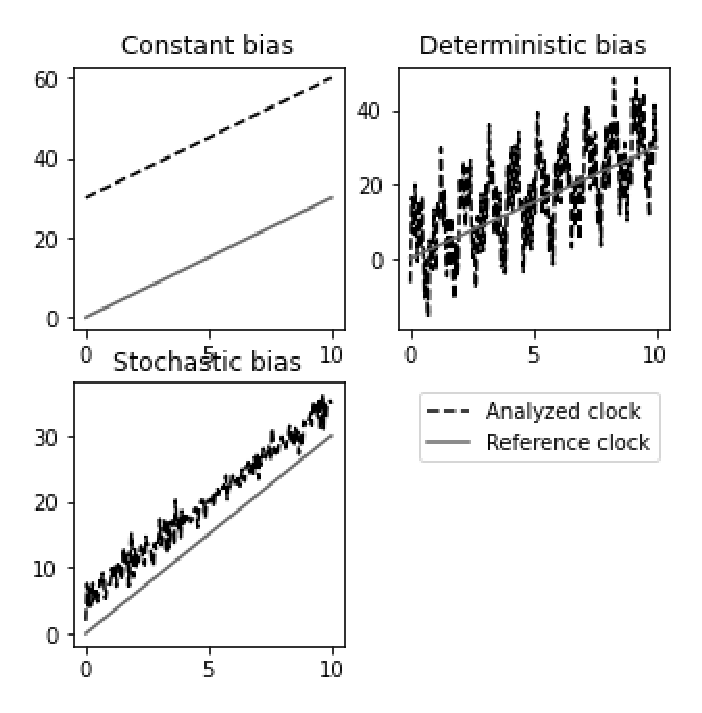
\includegraphics[width=\textwidth]{figures/bias_examples}
\caption{Example of clock readouts depending of nature of their bias}
\end{figure}
More information on exact clock and noise models will be given in following sections.

%----------------------------------------------------------------------------------------------------
\subsection{Basic clock model}
Basic clock model is a deterministic representation of clock as a second-order linear differential
equation.
\textbf{FIXME: MAKE ALL EQUATIONS USE SAME NOTATION}
\begin{equation}
	\label{equ:basic_clock}
	\ddot{x}(t)=z(t).
\end{equation}
Solution to that equation is
\begin{equation}
	\label{equ:basic_clock_solved}
	x(t)=x_{0}+y_{0}\tau+0.5z_{0}\tau^{2},
\end{equation}
where:
\begin{itemize}
	\item $x(t)$ is clock measurement at time $t$, also called time-offset or bias,
	\item $y(t)$ is fractional frequency offset,
	\item $z(t)$ is fractional frequency drift,
	\item $\tau$ is time difference defined as $\tau = t-t_{0}$.
\end{itemize}
Values $x_{0}$, $y_{0}$, $z_{0}$ refer to initial state of model at $t=t_{0}$.
Because frequency stability of clock degrades over time, as a result of ageing of physical 
components that they consist of, fractional frequency drift is sometimes called clock 
ageing parameter.
In this work $z(t)$ will be also referred to as the linear frequency drift. This terminology
was applied as in case of data used in this research there is a observable deterministic 
first order frequency drift behaviour.

%----------------------------------------------------------------------------------------------------
\subsection{Oscillator noise model}
Basic clock model is limited as it allows only for description of simple deterministic systems 
while real life implementations of clock are complex system with both deterministic and 
stochastic components. 
As described in section \ref{sec:physical_clock} of this chapter central element of every clock,
including atomic clocks, is an oscillator. That is why to create a more complex clock models 
an oscillator noise model must be created.
Role of this model is to derive a clock frequency and phase form an actual physical observation 
which in case of an atomic clock is voltage signal.
Equation describing voltage level on quartz oscillator, which is type of oscillator present in
atomic clocks, can be described by an equation:
\begin{equation}
	\label{equ:quartz_voltage}
	U(t)=(U_{0}+\epsilon(t))sin(2\pi \nu_{0}t + \phi(t)),
\end{equation}
where:
\begin{itemize}
	\item $U_{0}$ is peak voltage amplitude,
	\item $\nu_{0}$ is nominal frequency,
	\item $\phi(t)$ represents random phase deviations,
	\item $\epsilon(t)$ represents random amplitude deviations.
\end{itemize}
Since variation in signal amplitude do not influence measurements of signal frequency, save for
extreme cases where it drops so low that signal peak is not registered, it can be ignored in 
equation used for frequency stability analysis.
This means that equation actually used is:
\begin{equation}
	\label{equ:quartz_voltage_simplified}
	U(t)=U_{0}sin(2\pi \nu_{0}t + \phi(t)).
\end{equation}
Instantaneous clock frequency can be defined as the time derivative of the phase as demonstrated
on following equation:
\begin{equation}
	\label{equ:inst_frequency}
	\nu(t) = \nu_{0}+ \frac{1}{2\pi} \frac{d\phi}{dt},
\end{equation}
where $\frac{d\phi}{dt}$ represents instantaneous frequency offset.
The performance of the clock oscillator is determined by the frequency stability and not 
total frequency and the value of frequency offset is usually small in relation to measured.
Because of that it is more meaningful to describe clock stability with normalized, or fractional,
frequency as described in equation:
\begin{equation}
	\label{equ:normalized_frequency}
	y(t) = \frac{\nu(t)-\nu_{0}}{\nu_{0}} = \frac{dx}{dt}
\end{equation}
where
\begin{equation}
	\label{equ:what_is_time_offset}
	x(t) = \frac{\phi(t)}{2\pi \nu_{0}}
\end{equation}
is bias described in the units of time.


%----------------------------------------------------------------------------------------------------
\subsection{Standard clock model}



%====================================================================================================
\section{Stability analysis}

%----------------------------------------------------------------------------------------------------
\subsection{Allan variance}

%----------------------------------------------------------------------------------------------------
\subsection{Hadamard variance}

%----------------------------------------------------------------------------------------------------
\subsection{Sigma tau curves}


%====================================================================================================
\section{Modeling noise}

%----------------------------------------------------------------------------------------------------
\subsection{White phase modulation noise}

%----------------------------------------------------------------------------------------------------
\subsection{Flicker phase modulation noise}

%----------------------------------------------------------------------------------------------------
\subsection{White frequency modulation noise}

%----------------------------------------------------------------------------------------------------
\subsection{Flicker frequency modulation noise}

%----------------------------------------------------------------------------------------------------
\subsection{Random walk frequency modulation noise}

%----------------------------------------------------------------------------------------------------
\subsection{Oscilator noise as linear combination of power-law noises}

%----------------------------------------------------------------------------------------------------
\subsection{Sources of noise specific to orbital clocks}


%====================================================================================================
\section{State of the art in GPS clock bias prediction}

%----------------------------------------------------------------------------------------------------
\subsection{Time references in GPS}

%----------------------------------------------------------------------------------------------------
\subsection{Satellite broadcast polynomial}

%----------------------------------------------------------------------------------------------------
\subsection{IGU products}

\chapter{Machine learning based approach}


%====================================================================================================
\section{Concepts in machine learning}

%----------------------------------------------------------------------------------------------------
\subsection{Differences between knowlege and data based models}

%----------------------------------------------------------------------------------------------------
\subsection{What is a machine learning algorithm}

%----------------------------------------------------------------------------------------------------
\subsection{Deep learning}

%====================================================================================================
\section{Non neuron approaches}

%----------------------------------------------------------------------------------------------------
\subsection{Basics of regression}

%----------------------------------------------------------------------------------------------------
\subsection{Gradient approach}

%----------------------------------------------------------------------------------------------------
\subsection{Polynomial regression}

%----------------------------------------------------------------------------------------------------
\subsection{Gradient based adjustment}

%----------------------------------------------------------------------------------------------------
\subsection{Support vector machine}


%====================================================================================================
\section{Neural networks}

%----------------------------------------------------------------------------------------------------
\subsection{Feed forward neural networks}

%----------------------------------------------------------------------------------------------------
\subsection{Simple reccurent neural networks}

%----------------------------------------------------------------------------------------------------
\subsection{Networks with long term memory}


\chapter{Frequency analysis}

%====================================================================================================
\section{Frequency domain}

%----------------------------------------------------------------------------------------------------
\subsection{Fourier transform}

\subsubsection{Something}

\chapter{Machine learning in GPS clock bias prediction}


%====================================================================================================
\section{Review of research}

%====================================================================================================
\section{Data overview}

%====================================================================================================
\section{Linear regression baed approach}

%====================================================================================================
\section{Polynomial regression based approach}

%====================================================================================================
\section{Support vector regression based approach}

%====================================================================================================
\section{Neural network based approach}





\end{document}
